\documentclass[12pt, fleqn]{article}
\usepackage{../../../template/template}

%сам документ
\begin{document}
  \subfile{preamble.tex}
\section{Теория групп}
\subsection{Жордановы формы, 03.09.2019}

\begin{utv}
    Пусть $A \in M_n(\CC)$, $U \in GL_n(\CC)=\{U \in M_n(\CC): |U| \neq 0\}$

    Сопряжение матрицы A с помощью U: $A \longmapsto U^-1 A U$
\end{utv}

\begin{theorem}[Жордана, матрич. форма]
    $\forall A \e U: U^{-1} A U = J$\\
    Пусть $U^{-1} A U = J$, $V^{-1} A V = I$ - совпадают с точностью до перестановки жардановых блоков
\end{theorem}

\begin{example}
    $A_1 \in M_n(K)$, $A_2 \in M_m(K)$\\
    $\begin{pmatrix}
      A_1 & 0\\
      0 & A_2
    \end{pmatrix}$
    $\begin{pmatrix}
      A_2 & 0\\
      0 & A_1
    \end{pmatrix}$\\
    С помощью какой матрицы можно поулчить сопряжением другую
\end{example}

\begin{theorem}[Жордана, операт. форма]
    Пусть $L \in \mathscr{L}(V)$ (оператор на V), V - конечномерное пр-во над $\CC$. Тогда $\e \{e_1,...,e_n\}$ (жарданов базис) - базис V. $[L]_e=J$\\
    Единственность: если есть два базиса, то матрицы можно получить перестановкой
\end{theorem}
-------------- тут не хватает чего-то
\subsection{Собственные вектора, 10.09.2019}
------------- что-то пропущено\\
\subsection{Жордановы матрицы, 17.09.2019}

\begin{Example}
    \[A \in M_n(\CC)\]
    \[X^2=A=C^{-1}J C\]
    Пример $J=\begin{pmatrix}
      \lambda & 1\\
      0 & \lambda
    \end{pmatrix}$, $Y^2=J$, $Y=\begin{pmatrix}
      \sqrt{\lambda} & ?\\
      0 & \sqrt{\lambda}
    \end{pmatrix}$, ? - из уравнения
\end{Example}

Как найти J и C?

1) Находим все ссобственные числа матрицы A

Если все с.ч. равны, то J без единичек

Если одно собственное число
а) диагонализируема
$\begin{pmatrix}
\lambda & 0 & 0\\
0 & \lambda & 0\\
0 & 0 & \lambda
\end{pmatrix}$

б) блоки 2 и 1
$\begin{pmatrix}
\lambda & 1 & 0\\
0 & \lambda & 0\\
0 & 0 & \lambda
\end{pmatrix}$

в) $\begin{pmatrix}
\lambda & 1 & 0\\
0 & \lambda & 1\\
0 & 0 & \lambda
\end{pmatrix}$

\begin{example}
    Найдём, сколько собственных вектор-столбцов

    Первая матрица:
    $\begin{pmatrix}
    \lambda & 0 & 0\\
    0 & \lambda & 0\\
    0 & 0 & \lambda
    \end{pmatrix}
    \begin{pmatrix}
    x_1\\
    x_2\\
    x_3
    \end{pmatrix}
    =
    \begin{pmatrix}
    \lambda x_1\\
    \lambda x_2\\
    \lambda x_3
    \end{pmatrix}
    \Ra
    \begin{cases}
    \lambda x_1=\lambda x_1\\
    \lambda x_2=\lambda x_2\\
    \lambda x_3=\lambda x_3
    \end{cases}
    \Ra
    x_1,x_2,x_3 \in R
    $ - три л.н. переменные

    Для второго решение:
    $\begin{pmatrix}
    \lambda x_1\\
    0\\
    \lambda x_3
    \end{pmatrix}$ - 2 собственных вектор-столбца
\end{example}


\begin{example}
    Пусть у нас матрица 4*4, 2 собственных л.н. столбца (два блока)
\end{example}

\begin{utv}
    G,H - изоморфны, G - комм. $\Ra$ H - комм.
\end{utv}

\begin{proof}
    $\e \varphi: G \ra H: \varphi$ - биекция и $\varphi(g_1 g_2)=\varphi(g_1) \varphi(g_2)$, кроме того, $g_1 g_2=g_2 g_1$ $\forall g_1, g_2 \in G$, применим $\varphi$ к последнему выражению

    $h_1 h_2=\varphi(g_1) \varphi(g_2)=\varphi(g_1 g_2)=\varphi(g_2 g_1)=\varphi(g_2) \varphi(g_1)= h_2 h_1$
\end{proof}

\begin{homework}
    $X^2=\begin{pmatrix}
    0 & 1\\
    -1 & -1
    \end{pmatrix}$
\end{homework}

Дз: G,H - изоморфны, G - цикл. $\Ra$ H - цикл.
\begin{sol}
    Грппа G - цикл $\lra \e g \in G: \forall g' \in G \q \e k \in \Z$
    \[G \text{ - цикл., }G \cong H \Ra \e \varphi: G \ra H\]
    \[\forall h' \in H \q \e g' \in G: h'=\varphi(g')=\varphi(g^k)=\varphi(\underbrace{g...g}_k)=\underbrace{\varphi(g)...\varphi(g)}_k=\underbrace{h...h}_k=h^k\]
\end{sol}

Чтобы доказать, что две группы не изоморфны, можно доказать что у одной из них свойство выполняется, а у другой нет

\begin{example}
    \begin{enumerate}
        \item $\Z /_{6 \Z}$, $D_3$ - коммуннитативность
        \item $\Z /_{4 \Z}$, $\Z_{ /2 \Z} \times \Z /_{2 \Z}$ - цикличность
        \item $\Z /_{8 \Z}$, $\Z /_{4 \Z} \times \Z /_{2 \Z}$ - дз
        \item $\Z /_{4 \Z} \times \Z /_{2 \Z}$, $\Z /_{2 \Z} \times \Z /_{2 \Z} \times \Z /_{2 \Z}$ - порядки элементов
        \item $\Z$, $\Z \times \Z$ - цикличность?
    \end{enumerate}
\end{example}

\subsection{В ожидании кр..., 24.09.2019}

\begin{Example}
    \[A \in M_n(\CC),\q A=C^{-1}J C,\q C \in \Gl_n(\CC)\]
    \[J=
    \begin{pmatrix}
        \lambda& 1 &\ldots & 0\\
        0& \lambda &\ldots & 0\\
        \vdots& \vdots &\ddots & \vdots\\
        0&0 &\ldots & \lambda
    \end{pmatrix}\]
\end{Example}

1) находим все с.ч.

2) для каждого с.ч. находим л.н. уравнение

3) решаем систему линейных уравнений

...ЗДЕСЬ ЧТО-ТО ПРОПУЩЕНО, СМ. ТЕТРАДЬ

\begin{Example}
    \[D_3=\{e,l,r,s_1,s_2,s_3\}\]
    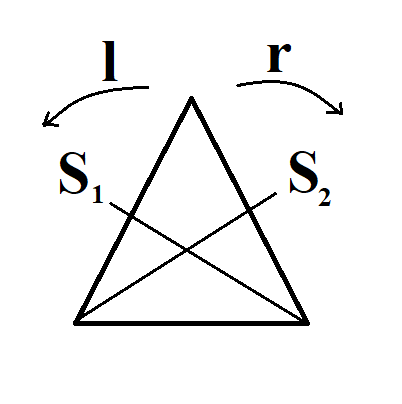
\includegraphics[scale=0.3]{triangle_d_3}
    \[H_1=\{e,r,l\}\]
    \[H_2=\{e,s_1\}\]
    1) Разбить по подгруппам, по левым и правым классам. Какая нормальная, какая нет?\\
    2) Найти g,G. Чтобы произведение не лежало в $H_2$
\end{Example}

Дз: $D_4=\{...\}$, $H_1=\{e,s_2\}$, $H_2=\{e, r^2\}$

Дз: $K(D_3)$ - найти коммутант для $D_3$

\subsection{Комутаторы и комутанты, 01.10.2019}

\begin{example}
  Дз (прошлое): $G=D_4$
  \[H=\{e,r^2\}\]
  \[H \triangleleft G\]
  \[G/_H\]
\end{example}

Дз (новое):
\begin{enumerate}
  \item Чему изоморфно $G/_H$? $\Z/_{4 \Z}$, $\Z/_{2 \Z} \times \Z/_{2 \Z}$
  \item $|G|=4 \ \Ra \
  \left[
  \begin{array}{ccc}
     G & \cong & \Z/_{4 \Z} \\
     G & \cong & \Z/_{2 \Z} \times \Z/_{2 \Z} \\
  \end{array}
\right.$
\end{enumerate}

\begin{example}[я не знаю, что это было]

\end{example}

\begin{example}
  \begin{enumerate}
    \item $\CC^* \ra \R^* \q (z \mapsto |z|)$
    \item $\CC^* \ra \CC^* \q (z \mapsto z^4)$

  \end{enumerate}
  Что получается при применении основной теоремы о гомоморфизме? (найти ядро образ, факторизовать, д-ть, что изморфна образу)
\end{example}

\begin{sol}
  \begin{enumerate}
    \item $\CC^*/_{\{Z \in \CC:\ |z|=1\}} \cong \R^*_{>0}$
    \item ДЗ
  \end{enumerate}
\end{sol}

\begin{example}
  ДЗ: $\GL_n(\R)/_{\{A \in \GL_n(\R):\ \det A = \pm 1 \}} \cong ?$

  Как это сделать? Нужно найти $\varphi: \GL_n(\R) \ra H$ - гомоморфизм: $\Ker \varphi = \{ A \in \Gl_n(\R):\ \det A = \pm 1\}$
\end{example}

\begin{Sol}
  \[\varphi(A)=|\det A|\]
  \[\varphi(A)=(\det A)^2\]
\end{Sol}

ДЗ: $\GL_n(\R)/_{\{A \in \GL_n(\R):\ \det A = \pm 1,\ \pm i \}} \cong ?$

\subsubsection{Действие группы на множество}

\begin{Example}
  \[D_4\]
  Написать разбиение этого множества из 16 эл-ов на орбиты. Сколько орбит?
\end{Example}

\begin{Sol}
  A
\end{Sol}

\subsection{Комутаторы и комутанты, 15.10.2019}

\begin{example}
  Грани кубика красят в три цвета, сколькими способами это можно сделать?
\end{example}

\begin{Proof}
  Группа - группа всех самосовмещений куба, сохраняющих ориентацию, она действует на множестве всех раскрасок фиксированного куба. Орбита - множество всех раскрасок фиксированного куба, которые можно получить его поворотом. Элементы G:
  \begin{enumerate}
    \item e - 1 шт.
    \item Поворот отн. оси, соединяющей центры противоположных граней на 90 градусов - 6 шт.
    \item ... на 180 - 3 шт.
    \item Поворот отн. диагонали на 120 градусов - 8 шт.
    \item Поворот отн. оси, соединяющей центры противоположных рёбер на 180 градусов - 6 шт.
  \end{enumerate}
  \[\Ra |G| = 24\]
  \[\text{Число орбит = }\dfrac{1}{|G|} \sum_{g \in G} |M^g|\]
  \[M^g = \{m \in M: gm = m\}\]
  \[= \dfrac{1}{24} \Br{\us{1.}{3^6} +
  \os{\text{4 одн. цв.}}{\us{2.}{6 \cdot 3^3}} +
  \os{\text{2 пр. одн. цв.}}{\us{3.}{3 \cdot 3^4}} +
  \os{\text{3 одн. цв.}}{\us{4.}{8 \cdot 3^2}} +
  \os{\text{2 одн. цв.}}{\us{5.}{6 \cdot 3^3}}} = 57\]
\end{Proof}
ДЗ 1: Аналогично, но красим в два цвета рёбра\\
ДЗ 2 (а): Есть ожерелье из 8 бусинок. Сколькими способами можно составить ожерелье из рубинов и алмазов\\
ДЗ 2 (б): если ограничение: должно быть 3 белых шарик и 5 черных

\subsubsection{Евклидовы пространства}
\begin{Example}
  \[\R[x]_3. \text{ Является ли это евклидовым пространством?}\]
  \begin{enumerate}
    \item $(f,g) = f(0) g(0) + f(1) g(1)$
    \item $(f,g) = f(0) g(0) + f(1) g(1) + 2 f(2) g(2)$
    \item $(f,g) = f(0) g(0) + f(1) g(1) + f(2) g(2) + 3 f(3) f(3)$
    \item $(f,g) = f(0) g(0) + f(1) g(1) + f(2) g(2) - f(3) f(3)$
  \end{enumerate}
\end{Example}

\begin{proof}
  \begin{enumerate}
    \item Не является, потому что для $f = x^2 - x$
    \[(f,f) = 0 \text{ - не работает}\]
    \item не является
    \item является
    \item
  \end{enumerate}
\end{proof}

\begin{example}
  Составить матрицу Грамма для в
  \[\text{Базис: }e_1 1,\q e_2 = x,\q e_3 = x^2,\q e_4 = x^3\]
  \[(x^2 - 1,\ x - 1)\]
\end{example}

\begin{proof}
  а
\end{proof}

\subsection{..., 22.10.2019}

ДЗ: ожирелье из 8 бусин: 4б, 4ч

\begin{Example}
  \[\R[x]_3,\q (f,g) = \int_0^1 fg dx\]
  Провести ортоганализацию Грамма-Шмидта в базисе $1, x, x^2, x^3$
\end{Example}

\begin{Sol}
  \[e_1 = 1 \text{ - готово}\]
  \[e_2 = x + \lambda \cdot 1 \q (e_2,\ 1) = 0\]
  Значит $\int\limits_0^1 (x + \lambda)\cdot 1 = \dfrac{x^2}{2} + \lambda x \Big|_0^1 = \dfrac{1}{2} + \lambda = 0 \Ra \lambda = -\dfrac{1}{2}$\\
  Должно быть $(e_2,\ e_2) = 1 \Ra \int\limits_0^1 (x^2 - 2 x\dfrac{1}{2} + \dfrac{1}{4}) = \dfrac{1}{3} - 2 \dfrac{1}{4} + \dfrac{1}{4} = \dfrac{1}{12}$
  \[\Ra e_2 = \dfrac{x - \dfrac{1}{2}}{\dfrac{1}{12}} = 12x - 6\]
  \[e_3 = x^2 + \lambda e_1 + \mu e_2 \q (e_3,\ e_2) = 0 \q (e_3,\ e_1)=0\]
  Значит $\int\limits_0^1$\\
  ДЗ: Найти $e_3,\ e_4$
\end{Sol}

\begin{Example}
  \[\R[x]_3,\q (f,g) = \int_0^1 fg dx\]
  В $V = <1,\ x>$ найти $\pr_V x^3$
\end{Example}

\begin{sol}
  По прошлой задаче $e_1 = 1,\ e_2 = 12x - 6$\\
  Значит $\pr_V x^3 = (x^3,\ 1) \cdot 1 + (x^3,\ 12x - 6) \cdot (12x - 6) =$\\
  $=\int\limits_0^1 x^3 + (\int\limits_0^1 12 x^4 - 6 x^3)(12x - 6) = \dfrac{1}{4} + (\dfrac{12}{5} + \dfrac{3}{2})(12x - 6) = $\\
  ДЗ: Проверить, что $u - pr_V u \bot v$
\end{sol}

\begin{Example}
  \[U = \R[x]_2,\q (f,g) = \int_0^1 fg dx\]
  В $V = <1,\ x>$, $Lf = f'$ найти $L^*$
\end{Example}

\begin{sol}
  ДЗ: досчитать
\end{sol}

\begin{example}
  Был пример $V = M_n(\R)$, там $(A,B) = \Tr AB^T$
  Найти в $V = M_n(\CC)$
\end{example}

\begin{Sol}
  \[\text{Проверим } (A,B) = \Tr A \ol{B}^T}\]
  \[\Tr \begin{pmatrix}
    a_1 & b_1\\
    c_1 & d_1
  \end{pmatrix} \begin{pmatrix}
    \ol{a_2} & \ol{b_2}\\
    \ol{c_2} & \ol{d_2}
  \end{pmatrix} = \Tr \begin{pmatrix}
    a_2 & b_2\\
    c_2 & d_2
  \end{pmatrix} \begin{pmatrix}
    \ol{a_1} & \ol{b_1}\\
    \ol{c_1} & \ol{d_1}
  \end{pmatrix}\]
  \[Tr \lambda\begin{pmatrix}
  a_1 & b_1\\
  c_1 & d_1
  \end{pmatrix} \begin{pmatrix}
    \ol{a_2} & \ol{b_2}\\
    \ol{c_2} & \ol{d_2}
  \end{pmatrix} = \lambda Tr \begin{pmatrix}
    a_1 & b_1\\
    c_1 & d_1
  \end{pmatrix} \begin{pmatrix}
    \ol{a_2} & \ol{b_2}\\
    \ol{c_2} & \ol{d_2}
  \end{pmatrix}\]
  ДЗ: на дом
\end{Sol}

\subsection{..., 29.10.2019}

ДЗ: Есть 2 оси и два угла. Нужно сделать повороты и найти итоговый поворот и понять, вокруг какой оси. Подсказка: в д-ве мы предъявляем ось, значит мы должны найти собственный вектор с с.ч. 1, т.е. нужно найти матрицу с базисом, например, в качестве осей. А можно выбрать базис для первого, потом для второго. А можно для обоих сразу. Пишем матрицу повортов и должны матрицы привести к одному базису. Когда найдем собственный вектор, берем ортоганальное дополнение. Смотрим, на какой угол поворачивает матрица. И нужно не забыть если это не стандартный базис, вернуть в стандартный базис.

\subsection{..., 05.11.2019}
ЧТО-ТО ПРОПУЩЕНО
\begin{Task}
  \[V= M_2(\R)\]
  \[(A,B) = \Tr AB^T\]
  \[LA=A^T\]
  Выяснить, про оператор L:
  \begin{enumerate}
    \item Самосопряженный?
    \item Ортогональный....?
  \end{enumerate}
\end{Task}

\begin{sol}
  \begin{enumerate}
    \item L - самосопр. $\lra$ $<LA,B>=<A,LB>$
    \[<LA, B> = \Tr(A^T B^T)\]
    \[<A, LB> = \Tr(A B)\]
    \[(AB)_{ij} = \sum_{k=1}^n a_{ik}b_{kj}\]
    \[(A^T B^T)_{ij} = \sum_{k=1}^n a_{ik}^T b_{kj}^T = \sum_{k=1}^n a_{ik} b_{kj}\]
    \[\Tr(AB) = \sum_{i=1}^n \sum_{k=1}^n a_{in} b_{nj}\]
    \[\Tr(A^T B^T) = \sum_{i=1}^n \sum_{k=1}^n a_{ki} b_{ik} = \sum_{k=1}^n \sum_{i=1}^n a_{ki} b_{ik}\]
    \[\Ra L \text{ - самосопр.}\]
    \item L - ортогон. т.и. т.т, когда $\Abs{A} = \Abs{LA}$
    \[\Abs{A}^2 = <A, A> = \Tr(A A^T) = \Tr(A^T A) = <LA, LA> = \Abs{LA}^2\]
  \end{enumerate}
\end{sol}

Выбрать произвольный ОНБ, считаем матрицу оператора (симм, ортог). Ищем базис из с.в.\\
ДЗ: ....\\
У самосопр. и ортог. оператора, есть базис, состоящий из собственных векторов. В нем матрица будет диагональная. На диагонали вещественные числа, по модулю равные $\pm 1$

\begin{task}
  Напишите не диагональную матрицу 2*2, которая положительно определена
\end{task}

\begin{Sol}
  \[\begin{pmatrix}
    x_1 & x_2
\end{pmatrix}\begin{pmatrix}
    2 & 1\\
    1 & 2
  \end{pmatrix} \begin{pmatrix}
    x_1\\
    x_2
  \end{pmatrix} = 2x_1^2 + x_1 x_2 + x_1 x_2 + 2x_2^2 = x_1^2 + x_2^2 + (x_1 + x_2)^2 \os{\forall x \neq 0}{>} 0\]
\end{Sol}

\begin{task}
  Напишите не диагональную матрицу 2*2, которая положительно полуопределена, не положительно определена. Убедиться в этом по всем критериям
\end{task}

\begin{Sol}
  \[\begin{pmatrix}
    ? & ?\\
    ? & ?
  \end{pmatrix}\]
\end{Sol}

ДЗ: Найти ту матрицу P из док-ва

\subsection{Квадратичные формы, 12.11.2019}

\begin{task}
  Написать положительно определенную матрицу от двух переменных с отрицательными коэффициентами
\end{task}

\begin{Sol}
  \[A(x,y)=\begin{pmatrix}
    x^2 & -y^2\\
    -y^2 & x^2
  \end{pmatrix}\]
  Удовлетворяет критерию Сильвестра
\end{Sol}

\begin{task}
  Преобразовать к каноническому виду ортоганальным прелбразованием $2x_1^2 + x_2^2 - 4x_1 x_2 - 4x_2 x_3$
\end{task}

\begin{Reminder}
  \[S(x) = \sum \us{b_{ij} = b_{ji}}{a_{ij} x_i x_j}\]
  \[b_{ij} = \left[\begin{matrix}
    a_{ij}, & i=j\\
    \frac{a_{ij}}{2}, & i > j\\
    \frac{a_{ji}}{2}, & j>i
  \end{matrix}\right.\]
\end{Reminder}

\begin{Sol}
  \[\begin{pmatrix}
    2 & -2 & 0\\
    -2 & 1 & -2\\
    0 & -2 & 0
  \end{pmatrix} \text{ - не пол. опр. по критерию Сильвестра}\]
  Найдем собственные числа этой матрицы:
  \[\begin{vmatrix}
    2 - \lambda & -2 & 0\\
    -2 & 1 - \lambda & -2\\
    0 & -2 & 0 - \lambda
  \end{vmatrix} \Ra \lambda_1 = 1\q \lambda_2 = -2\q \lambda_3 = 4\]
  Подставим в какноническую форму:
  \[Q(x) = x_1^2 - 2x_2^2 + 4x_3^2\]
  Чтобы найти соответствующее линейное преобразование, нужно найти собственные вектора:
  \[\begin{cases}
    (2-1)x + -2y = 0\\
    -2x + (1-1)y -2z = 0\\
    -2y -z = 0
  \end{cases} \Ra (x,y,z) = (,,)\]
  \[\begin{cases}
    (2+2)x + -2y = 0\\
    -2x + (1+2)y -2z = 0\\
    -2y +2z = 0
  \end{cases} \Ra (x,y,z) = (,,)\]
  \[\begin{cases}
    (2-4)x + -2y = 0\\
    -2x + (1-4)y -2z = 0\\
    -2y - 4z = 0
  \end{cases} \Ra (x,y,z) = (,,)\]
\end{Sol}

\end{document}
